\documentclass{article}
\usepackage{hyperref}
\usepackage{tikz}
\usepackage{pgfplots}

\author{Nicolas Loza}
\title{ESTAData - Algorithms and Data Structures}
\date{}
\begin{document}
	\maketitle
	\section{Introduction}
		This document serves as documentation of the java implementation of the spatio-temporal 
		clustering framework proposed in \cite{BBTRB}, under the scope of the ESTAData project,
		directed by \href{https://scholar.google.com/citations?user=IUoh6nMAAAAJ}{Julio Borges}. 
		Therefore, it is recommended for the readers to be familiar with the 
		terms and definitions presented in \cite{BBTRB}. Moreover, the framework uses the Terracotta
		library for data storage and management. Thus, the reader should also bring basic knowledge
		of how said library works. Finally, the code corresponding to this documentation can be found 
		in the repository \url{https://github.com/aqnmd/ESTAData}.
				
		
	\section{Overview}
		This section provides a quick overview of the project's packages and the functionalities they
		provide.
		\begin{itemize}	
			\item \texttt{Default}: only the entry point class \texttt{Mining.java} is provided, which
				parses the input provided through the console and interprets it accordingly.
			\item \texttt{de.estadata.mining.datatransformation}: contains three important classes:
			\begin{itemize}	
				\item \texttt{BigMemory.java}: instantiates the Terracotta CacheManager.
				\item \texttt{Report.java}: represents a report, thus containing properties like coordinates, timestamps and description, among others.
				\item \texttt{Cluster.java}: represents a set of Reports that have been clustered together (how is not specified).
			\end{itemize}
			\item \texttt{de.estadata.mining.gephiextension}: contains classes that fix minor bugs found in the Gephi library.
			\item \texttt{de.estadata.mining.graphmodel}: models the graph structure used by all of the framework's algorithms. Consists of:
			\begin{itemize}	
				\item \texttt{Node.java}: models a single node in the graph (that corresponds to a single report).
				\item \texttt{Edge.java}: models an edge between two nodes (meaning the respective reports are ST-connected).
				\item \texttt{Graph.java}: manages the sets of nodes and edges by storing them in separate Terracotta Caches.
				\item \texttt{GraphView.java}: models a 'view' of the graph by containing a subset of the graph's nodes and/or a subset of its edges.
			\end{itemize}
			\item \texttt{de.estadata.mining.modularityoptimizer}: provides a set of modularity based clustering algorithms. It is an adaptation of the
				code provided in \url{http://www.ludowaltman.nl/slm/}.
			\item \texttt{de.estadata.mining.scan}: provides a single class \texttt{SCAN.java} implementing the algorithm of the same name on the 
				previously mentioned graph structure.
			\item \texttt{de.estadata.mining.util}: provides utility functionalities divided in two classes:
			\begin{itemize}
				\item \texttt{DataLoader.java}: is the class that allows the loading of reports data from .csv and .json files.
				\item \texttt{MiningTools.java}: is a class providing a wide range of methods that are used throughout the 
					framework, but can also be useful for external users of the library.
			\end{itemize}
		\end{itemize}
		
		The project is also provided in form of a jar file, which can be used directly to execute most
		of the functionalities made available by the packages mentioned above. We will refer to this
		file from now on as ``\texttt{mining.jar}'', and in the following sections will provide examples
		of how to used under different circumstances and for different purposes.
	
	\section{Data Loading}
	\label{data loading}
		Once Terracotta has been correctly set up (see [TODO: add terracotta reference]), we can 
		proceed to the first step: loading the data into Terracotta Caches. Using \texttt{mining.jar} this
		is quite straightforward:\\ \\
		\texttt{\$ java [JVM args] -jar mining.jar --config CONFIG\_FILE --reportscache CACHE --load PATH --type [json|csv] --ratio R} \\ \\
		As we will see in future sections, the JVM arguments tend to have a big impact in the performance 
		of the framework. Especially, when loading big datasets, the JVM should have access to 
		as much memory as possible. This is done using the flag \texttt{-Xmx} (e.g. 
		\texttt{-Xmx8G} will allow the JVM heap to use up to 8G of memory).\\
		Regarding the program arguments
		\begin{itemize}
			\item CONFIG\_FILE is the path to the Terracotta configuration file,
			\item CACHE is the name of the Terracotta cache where the reports should be stored in,
			\item \texttt{PATH} is the path to a directory or single file containing the data 
				(must be \texttt{json} or \texttt{csv}),
			\item and the ratio \texttt{R} is a parameter in range $[0,1]$ signalizing which 
				percentage of the data should be loaded. Its default value is 1.0, and if minor to 
				one, the selected data is random (i.e. two executions using the same ratio could 
				result in different sets of data being loaded).
		\end{itemize} 
		It is worth noting that the flags \texttt{--config} and \texttt{--reportscache} are not 
		specific to the load functionality, but must \emph{always} be provided when using 
		\texttt{mining.jar} from the command line.\\
		In case of using the framework as a library, the same functionality is available under the 
		aforementioned class \texttt{DataLoader}, which provides a single static method
		\texttt{load(String dataType, String dataPath, Cache reportsCache, double ratio)}. The names
		of the arguments represent the same as the above command line arguments.\\
		In order to successfully load the information from the csv/json files, they need to provide 
		certain information. Otherwise, the load functionality ends in failure. This is avoided
		if the data files contain the following columns with their respective values:
		\begin{itemize}
			\item 'lng' for longitude (a double precision floating point number).
			\item 'lat' for latitude (a double precision floating point number).
			\item 'created\_at' for the creation time of the report. For .csv files, 
				the date formatting should be 'yyyy-MM-dd HH:mm:ss', for .json files: 
				'yyyy-MM-dd'T'HH:mm:ss' (a string).
			\item 'summary' for the category of the report (a string).
			\item 'description' for the user's description of the report (a string).
			\item for the report's URL address, 'bitly' in case of .csv files, 
				'html\_url' in case of .json files (a string).
			\item 'id' for the report's ID (an integer).
			\item in case of .json files, 'reporter' for the ID of the reporter (an integer).
		\end{itemize}
		
	\section{Graph generation}
	\label{graph generation}
		Because of the nature of the different analysis provided in the framework, we first need to
		generate a graph from the set of reports previously loaded into the cache. Fortunately, this
		process is mostly automatized and can be called in a single command line:\\
		\texttt{\$ java [JVM args] -jar mining.jar [\emph{config+cache}] --mode filter -m M -d D}\\
		As when loading data into Terracotta, it is important to provide the JVM with as much heap 
		memory (flag \texttt{-Xmx}) as well as with off-heap memory (flag \texttt{-XX:MaxDirectMemorySize}).
		Regarding the program arguments:
		\begin{itemize}
			\item \texttt{\emph{config+cache}}: here, the configuration file of terracotta and the 
				cache containing the reports needs to be provided (see \ref{data loading}). However,
				a further cache is also needed. In it, the clustering results are to be stored.
				This cache is provided using the flag \texttt{--clusterscache}.
			\item \texttt{--mode filter} indicates the modality being executed. In future sections we shall see the alternatives.
			\item \texttt{-m M} or \texttt{--meters M} indicates the maximal spatial distance M in meters 
				that two reports can have to be ST-connected.
			\item \texttt{-d D} or \texttt{--days D} indicates the maximal temporal distance D in days
				that two reports can have to be ST-connected.
		\end{itemize}
		The successful execution of this command line has the following results:
		\begin{itemize}
			\item Two new caches generated containing the information concerning the graph structure. These are named
				\texttt{[reportsCache]\_nodesCache} and \texttt{[reportsCache]\_edgesCache}. Thus, if the
				cache containing the reports is called \texttt{NYC}, the new caches are called 
				\texttt{NYC\_nodesCache} and \texttt{NYC\_edgesCache}. As we can see from their names, 
				the first cache contains the graph's nodes and the second one its edges.
			\item Each node in the graph represents a single report, and an edge between two nodes 
				means they are ST-connected under the provided parameters.
			\item Once the graph has been generated, each of its connected components is assigned 
				a unique, positive cluster ID (isolated nodes are assigned the cluster ID -1).
			\item Once every node in the graph has a cluster ID, they are grouped in \texttt{Cluster}
				objects according to their cluster ID. These \texttt{Cluster} instances are then
				stored in the corresponding Terracotta cache.
		\end{itemize}
		When using the framework as library, the same functionality is provided by the class 
		\texttt{STFiltering}. Unlike the command line version of the framework, the usage of this
		class to achieve the same results as the ones listed above requires several steps. We 
		shall now provide an overview of the class' constructor and methods, and then some examples
		as how to use them.\\
		When creating an instance of \texttt{STFiltering}, there are three possible ways to do so:
		\begin{enumerate}
			\item \texttt{STFiltering(List<Integer> reportIDs, CacheManager databaseManager,
				Cache reportsCache, int maxSpaceDist, int maxDayDist)}
			\item \texttt{STFiltering(CacheManager databaseManager, Cache reportsCache,
			int maxSpaceDist, int maxDayDist)}
			\item \texttt{STFiltering(CacheManager databaseManager, Cache reportsCache,
			boolean useExistingGraphStructure)}
		\end{enumerate}
		All of these constructors result in the generation of the graph's \texttt{Node} instances, but 
		\emph{not} the \texttt{Edge} instances (this takes place in a later step)\footnote{Despite
		the edges not being yet generated, the corresponding \texttt{Cache} instances for nodes and edges
		are generated after the execution of each constructor.}. As with the command
		line version, a Terracota \texttt{CacheManager} and a \texttt{Cache} need to be provided for
		the graph generation. Each constructor, however, offers a slightly different functionality.
		The first one allows its caller to specify a list of the report IDs to be used for the graph 
		generation (i.e. every report whose ID is not contained in the list is ignored).
		The second one does not take any list of IDs and works with all the reports present in the provided
		cache. The third constructor has different behaviours depending on its third argument: 
		if it is set to \texttt{true}, the program attempts to recover a previously generated 
		graph instance corresponding to the given \texttt{Cache}. In this case, the respective 
		caches for nodes and edges should exist under the given \texttt{CacheManager} and be named 
		as previously specified. On the other hand, if the third parameter is set to
		\texttt{false}, the program reads all reports from the given cache and generates a graph using
		standard values for spatial and temporal distance: 100 meters and 30 days, respectively.\\
		There is a very particular side-effect from running any of this constructors, except for the
		third one for recovering a previously generated graph. Namely: the program generates a set 
		of temporary Terracotta caches (hereafter referred to as ``buckets''). 
		How many, depends on the total time span of the reports and 
		on the maximal temporal distance two reports may have. More precisely\footnote{Because 
		$timeSpan$ is given in milliseconds, $maxDayDist$ must also be translated to
		milliseconds.}:
			$$timeSpan = endTime - startTime$$
			$$\#buckets = \left\lceil \frac{timeSpan}{maxDayDist} \right\rceil$$
		These buckets store information about the reports and help in the generation of the graph's
		edges, which is the next step after constructing the instance. This is achieved by calling the 
		method \texttt{void generateGraph()}. More importantly, because of the algorithms quadratic complexity,
		the buckets help avoiding the worst case scenario of comparing each node to every other node
		in search for possible ST-connections. Instead, only nodes that are in close temporal proximity
		are compared with one another. Hence the creation of the buckets. Moreover, because the set
		of report references contained in each bucket is disjoint with every other bucket, this allows 
		a very effective parallelization of the algorithm. For specific results, see \ref{evaluation}. 
		Finally, once the graph's edges have been generated (i.e. once the 
		execution of \texttt{generateGraph()} is finished), all buckets are disposed of.\\
		After generating the graph, one can directly proceed to generate the clusters from the 
		graph's connected components and transfer them to a separate \texttt{Cache}. This is done
		by calling the method with the signature \\
		\texttt{void generateAndTransferClusters(Cache clustersCache)}.	Note that this method 
		clears any previous data stored in the \texttt{Cache} passed as argument
		and writes its results. However, the class also offers an alternative method called 
		\texttt{void generateAndTransferClusters(Cache clustersCache, GraphView view)}, which does has
		the same behaviour as the previous one, except that it only clusters nodes and edges whose IDs are 
		contained in the passed \texttt{GraphView}.\\
		Such a view can be generated using the method \texttt{GraphView filter(double newMaxSpaceDist, 
		int newMaxDayDist, boolean mustShareCategory)}, which allows its caller to execute a filtering
		over the graph's edges with more strict parameters as the ones used for generating it. The
		resulting view contains all of the graph's node IDs, but only the edge IDs of those edges that 
		fulfil the more strict 	parameters.
	
	\section{Graph clustering}
	\label{graph clustering}
		Once the graph has been generated (see \ref{graph generation}), the framework also allows the 
		usage of known clustering algorithms for the refinement of the clusters given by the graph
		in a first instance (which are simply its connected components). From the command line, these
		algorithms can be executed as follows:\\ \\
		\texttt{\$ java [JVM args] -jar mining.jar [\emph{config+caches}] --mode cluster --algorithm ALG [ARGS]}\\ \\
		Like in \ref{graph generation}, the JVM arguments should assign the as much memory (on- and off-heap)
		as possible to the program. Just as well as before, \texttt{\emph{config+caches}} contains 
		the necessary information about the Terracotta configuration file and the caches containing 
		the reports and clusters. As in some cases of the previous section, in this scenario we need 
		a graph to work on. Therefore, the necessary caches should exist with the convention names 
		(see \ref{graph generation} for further information).\\
		Regarding the remaining arguments, \texttt{--mode cluster} indicates that the program must 
		execute a clustering algorithm over the (presumably existent) graph; \texttt{ALG} is the
		algorithm to be executed, which can be one of the following: \texttt{scan} (for the algorithm 
		of the same name, see \cite{X07}), \texttt{louvain}, \texttt{louvain\_mlv} (for Louvain with 
		multilevel refinement) or \texttt{slm} (for smart local moving algorithm for large-scale 
		modularity-based community detection). The last three are modularity based algorithms, and 
		their provided implementations were taken from \url{http://www.ludowaltman.nl/slm/}.\\
		When using SCAN, \texttt{ARGS} consists of: \texttt{--mu MU --eps EPS}, which are the 
		algorithm's parameters as described in \cite{X07}. If not provided, \texttt{MU} and \texttt{EPS}
		take the default values $2$ and $0.7$, respectively.\\
		On the other hand, when using any of the modularity based algorithms, a wide set of arguments
		is available for the user. 
		\begin{itemize}
			\item \texttt{--modularity\_function FUNC}: the modularity function to be used (\texttt{standard} (default) or \texttt{alternative}).
			\item \texttt{--resoltion RESOL}: the resolution parameter (default: $1.0$).
			\item \texttt{--random\_starts RANDS}: the number of random starts executed by the algorithm, default: $10$.
			\item \texttt{--iterations ITER}: the number of iterations per random start, default: $10$.
			\item \texttt{--random\_seed SEED}: seed for the RNG, default: random.
		\end{itemize}
		For more detailed information about these arguments, we refer to the aforementioned website.\\ \\
		When using the framework as library, the same functionalities are made available by the class
		\texttt{GraphClustering}. In order to use it, one needs to instantiate it by calling
		\texttt{GraphClustering(graph, pointsCache, clustersCache)}. The specific
		algorithms are run either by calling \texttt{void runSCAN(epsilon, mu)} to run SCAN, or
		by calling 
		\texttt{void runModularityOptimizer(modFunc, resolution, algorithm, randomStarts, 
		iterations, randomSeed)} for any of the other three algorithms. Finally, once the 
		chosen algorithm has finished its execution, \texttt{generateAndTransferClusters()}
		allows the generation of \texttt{Cluster} instances and their storage in the respective
		\texttt{Cache}.
	\section{Evaluation}
	\label{evaluation}
		This section consists of a set of results after using the framework over different datasets. 
		Moreover, we compare the framework against running the same algorithm but without the underlying
		data management from Terracotta (i.e. by maintaining all objects in the java heap).\\
		The following are results obtained after executing our implementations in an amazon server
		running Ubuntu 12.04. The machine ran with 8 Intel(R) Xeon(R) CPU E5-2680 v2 @ 2.80GHz CPUs (2 threads per core)
		and 16GB of RAM. Every experiment was executed with as few programs running in the background 
		as possible.\\
		The running times plotted in the two graphs below compare the running time necessary for the 
		generation of the graph structure (i.e. generation of nodes for each report and the computation
		of the ST-connections between them). In the first plot, we can see that the running times differ
		in very little, which may actually be caused by the overhead of getting information from the
		Terracotta caches (otherwise, the algorithms are identical). However, when analysing a
		dataset with close to 3 million reports, both frameworks exited with a GC Overhead Exception.
		
			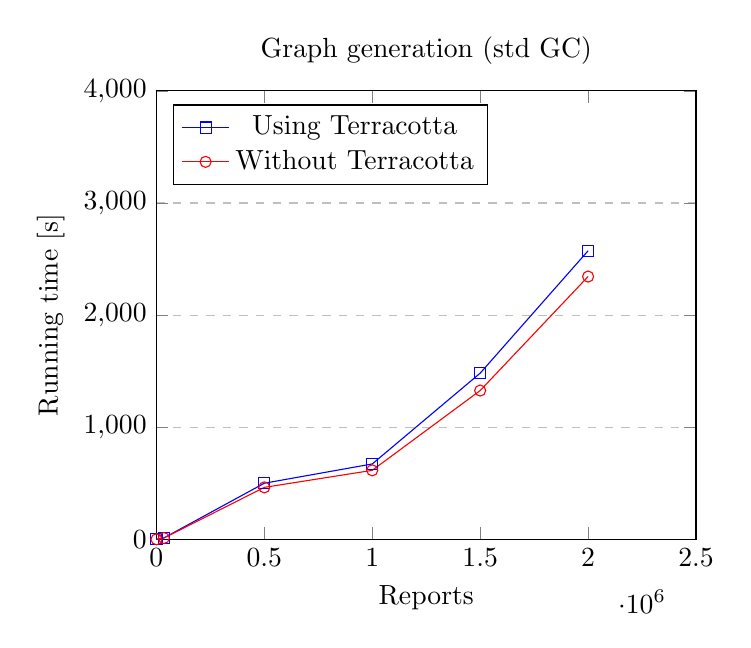
\begin{tikzpicture}
				\begin{axis}[
					title={Graph generation (std GC)},
					xlabel={Reports},
					ylabel={Running time [s]},
					xmin=0, xmax=2500000,
					ymin=0, ymax=4000,
					legend pos=north west,
					ymajorgrids=true,
					grid style=dashed,
				]
				 
				\addplot[
					color=blue,
					mark=square,
					]
					coordinates {
					(432,0.120)(34690,12)(500000,500)(1000000,672)(1500000,1482)(2000000,2574)
					};
					\addlegendentry{Using Terracotta}
					
				\addplot[
					color=red,
					mark=o,
					]
					coordinates {
					(432,0.043)(34690,11)(500000,463)(1000000,615)(1500000,1327)(2000000,2344)
					};
					\addlegendentry{Without Terracotta}
				 
				\end{axis}
			\end{tikzpicture}
	
			Because of the before mentioned GC Overhead, we attempted to run both frameworks again, this
			time using a more efficient Garbage Collection Algorithm, which takes advantage of the 
			multiple cores available. The results can be seen in the second plot. Using this configuration,
			the running times up to the 2 million reports did not differ much from the ones with the
			original configuration using the standard Garbage Collector. However, we were able to 
			successfully analyse the dataset with 3 million reports, although with quite different
			results: the framework running without Terracotta is almost twice as fast as the
			one using it. This may lie in the configuration of the Terracotta Caches. A change of
			strategy in the usage of the Caches of Terracotta, or a more in-depth approach to the
			configuration of these seem to be the options to optimize the results.
	
			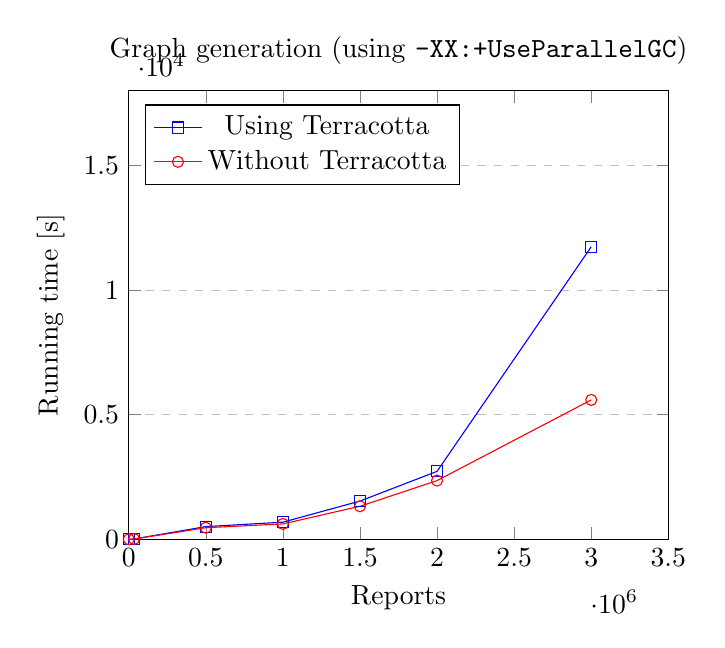
\begin{tikzpicture}
				\begin{axis}[
					title={Graph generation (using \texttt{-XX:+UseParallelGC})},
					xlabel={Reports},
					ylabel={Running time [s]},
					xmin=0, xmax=3500000,
					ymin=0, ymax=18000,
					legend pos=north west,
					ymajorgrids=true,
					grid style=dashed,
				]
				 
				\addplot[
					color=blue,
					mark=square,
					]
					coordinates {
					(432,0.128)(34690,12)(500000,509)(1000000,686)(1500000,1534)(2000000,2727)(3000000,11745)
					};
					\addlegendentry{Using Terracotta}
					
				\addplot[
					color=red,
					mark=o,
					]
					coordinates {
					(432,0.058)(34690,10)(500000,464)(1000000,616)(1500000,1325)(2000000,2356)(3000000, 5595)
					};
					\addlegendentry{Without Terracotta}
				 
				\end{axis}
			\end{tikzpicture}

	\begin{thebibliography}{9}
		\bibitem{BBTRB}
			Budde, M., Borges, J. D. M., Tomov, S., Riedel, T., \& Beigl, M. Improving Participatory Urban Infrastructure Monitoring through Spatio-Temporal Analytics.
		\bibitem{X07}
			Xu, Xiaowei, et al. ``Scan: a structural clustering algorithm for networks''. Proceedings of the 13th ACM SIGKDD international conference on Knowledge discovery and data mining. ACM, 2007.
	\end{thebibliography}
\end{document}